\documentclass[conference,final]{IEEEtran}
\usepackage{latex8}
\usepackage{times}

\usepackage[utf8]{inputenc}
\usepackage{graphicx}
\usepackage{url}
\usepackage{float}
\usepackage{times}    
\usepackage{multirow}    
\usepackage{listings}   
\usepackage{times}     
\usepackage{paralist}    
\usepackage{wrapfig}    
\usepackage[small,it]{caption}
\usepackage{multirow}
\usepackage{ifpdf}


\usepackage{listings}
\usepackage{keyval}  
\usepackage{color}
\definecolor{listinggray}{gray}{0.95}
\definecolor{darkgray}{gray}{0.7}
\definecolor{commentgreen}{rgb}{0, 0.4, 0}
\definecolor{darkblue}{rgb}{0, 0, 0.4}
\definecolor{middleblue}{rgb}{0, 0, 0.7}
\definecolor{darkred}{rgb}{0.4, 0, 0}
\definecolor{brown}{rgb}{0.5, 0.5, 0}

\lstdefinestyle{myListing}{
  frame=single,   
  backgroundcolor=\color{listinggray},  
  %float=t,
  language=C,       
  basicstyle=\ttfamily \footnotesize,
  breakautoindent=true,
  breaklines=true
  tabsize=2,
  captionpos=b,  
  aboveskip=0em,
  belowskip=-2em,
  %numbers=left, 
  %numberstyle=\tiny
}      

\lstdefinestyle{myPythonListing}{
  frame=single,   
  backgroundcolor=\color{listinggray},  
  %float=t,
  language=Python,       
  basicstyle=\ttfamily \footnotesize,
  breakautoindent=true,
  breaklines=true
  tabsize=2,
  captionpos=b,  
  %numbers=left, 
  %numberstyle=\tiny
}

\newcommand{\up}{\vspace*{-1em}}
\newcommand{\upp}{\vspace*{-0.5em}}
\newcommand{\numrep}{8 }
\newcommand{\samplenum}{4 }
\newcommand{\tmax}{$T_{max}$ }
\newcommand{\tc}{$T_{C}$ }
\newcommand{\bj}{BigJob}

\title{Scaling-Out MapReduce: From High-Performance Distributed
  Resources to Web-Scale Resources}

\author{ Miklos Erdelyi$^4$, Saurabh Sehgal$^5$, Andre Merzky$^1$,
  \newline Shantenu Jha$^{123*}$ \\
  \small{\emph{$^{1}$Center for Computation \& Technology, Louisiana State University, USA}}\\
  \small{\emph{$^{2}$Department of Computer Science, Louisiana State University, USA}}\\
  \small{\emph{$^{3}$e-Science Institute, Edinburgh, UK}}\\
  \small{\emph{$^{4}$Department of Computer Science, University of
      Pannonia, Veszprem, Hungary}}\\
 \small{\emph{$^{5}$ Edward S. Rogers Sr. Department of Electrical and Computer Engineering  University of Toronto}}\\
 \small{\emph{$^{*}$Contact Author: \texttt{sjha@cct.lsu.edu}}}\\
}

%\date{}

\def\acknowledgementname{Acknowledgements}
\newenvironment{acknowledgement}%
{\section*{\acknowledgementname}%
\parindent=0pt%
}

\newif\ifdraft
%\drafttrue
\ifdraft
\newcommand{\llnote}[1]{ {\textcolor{green} { ***JK: #1 }}}
\newcommand{\alnote}[1]{ {\textcolor{blue} { ***AL: #1 }}}
\newcommand{\jhanote}[1]{ {\textcolor{red} { ***SJ: #1 }}}
\else
\newcommand{\llnote}[1]{}
\newcommand{\alnote}[1]{}
\newcommand{\jhanote}[1]{}
\fi

\begin{document} 

\maketitle    

\begin{abstract}
  Scale-out means: Using multiple concurrent distributed resources
  across scales, e.g., small clusters to HPC resources.  The aim of
  this paper is to (i) define, develop and validate a scale-out
  verison of MapReduce across clusters, clouds and HPC resources. (ii)
  To show how SAGA enables the use of MapReduce and related
  programming models -- Sphere (yes), Dryad (this is via diggedag).
  (iii) To provide the basis for supporting dynamic data-intensive
  applications viz., diggedag and simple tests to show the concepts
  and suggest that this needs to be implemented in the context of
  MapReduce too. \jhanote{SJ to elaborate}
\end{abstract}

\up
\section{Introduction}
\up

There are numerous scientific applications that utilize data and
resources distributed over vast heterogeneous infrastructures and
networks with varying speeds and characteristics. However, despite the
drastic differences in hardware capabilities of such distributed
systems, applications usually tend to utilize a single infrastructure
for all of their computational and data processing needs. Since most
distributed frameworks are designed with specific assumptions and
infrastructures in mind, dependence on a single technology in a
heterogeneous environment is not always an optimal choice to gain
maximum runtime performance. For example, the Sector/Sphere data cloud
is exclusively designed to support data-intensive computing on high
speed networks, while other distributed filesystems like GFS/Hadoop
assume limited bandwidth among infrastructure nodes [1]. Thus, for
applications to efficiently utilize heterogeneous environments,
abstractions must be developed for the efficient utilization of and
orchestration across such distinct distributed infrastructure.  SAGA
or “Simple API for Grid Applications” is a high level API that
provides a simple, standard and uniform interface to the most commonly
required distributed functionality [2]. SAGA can be used to encode
grid applications, tool-kits to manage distributed applications as
well as implement abstractions that support commonly occurring
programming, access and usage patterns. Popular programming
abstractions such as Map-Reduce and All-Pairs have been successfully
implemented with SAGA to showcase its utilization as a flexible
framework to scale-out data-intensive computations on different
flavours of grids and clouds, and attain a high level of
interoperability at the application level. Thanks to the ease of
developing SAGA “Adaptors”, developers can provide SAGA the interfaces
to interact with widely different infrastructures simultaneously
throughout the execution of a single application.

This paper reports on progress on three-fronts: First, we take the
existing SAGA Map-Reduce implementation, and enhance it to increase
performance and ease of use for application programmers through adding
features such as serialization and compression of intermediate data,
ability to define a combiner function to reduce network traffic and
data-locality optimization at task assignment.  Secondly, we develop a
SAGA adaptor for the Sector/Sphere compute and data cloud. The adaptor
translates the high level SAGA job submission and file manipulation
APIs into Sector/Sphere operations. This allows SAGA applications to
leverage the functionality provided by the Sector/Sphere cloud for
processing large data sets on infrastructures with high speed
networks.  The third is the creation of components that facilitate
flexibility in data placement relative to the computational resource
-- that is either data can be transferred intelligently to match
computational workloads or computational workloads can be placed to
match (prevent) data requirements. More generically, it is worth
mentioning that these approaches can be extend to support certain
kinds of {\it affinities}.

{\it Enhancing SAGA-based Map-Reduce Performance:} To orchestrate the
functioning of the various different frameworks, we use the
master-worker programming pattern, on which the SAGA Map-Reduce
implementation is also based. This pattern allows the workers to
execute on the different infrastructures (including Sector/Sphere)
while communicating their progress and results through an advert
database to the master~\cite{saga_ccgrid09}. The performance
enhancements to the existing SAGA Map-Reduce implementation come
partly from reduced network bandwidth usage and partly from more
efficient processing when reading or writing serialized data by the
workers. Network traffic is primarily reduced by applying
data-locality optimization: the master tries to assign chunks of the
input to workers such that the data to be processed will reside near
or on the worker node itself, thus avoiding the need for transferring
data blocks by the distributed filesystem implementation. Information
for this decision is obtained by the master through SAGA's "Replica"
interface. The amount of network usage is further reduced when the
user specifies a combiner function which is then used for aggregating
key/values locally on the worker. The processing of input and output
key/value pairs is enhanced by minimizing expensive memory I/O
operations.

{\it Sector/Sphere Adaptors: }Sphere represents a programming paradigm
that is different from MapReduce, and allows for a more general and
wider approach to performing data intensive computations. Instead of
using the more specific map/reduce implementations, an application can
define any arbitrary functions to operate on data stored in the Sector
cloud at multiple levels[1]. The Sector/Sphere adaptor drives the
translation of the SAGA job submission APIs into executing the User
Defined Functions or UDFs through Sphere on the Sector data cloud.
Specifically, the Sector/Sphere adaptor in conjunction with others
(KFS, HDFS, Amazon EC2) naturally give us the opportunity to
experiment with various distinct frameworks running on infrastructures
best suited for their purposes. The SAGA MapReduce implementation
utilizes these adaptors to submit jobs to the underlying heterogeneous
infrastructure. With the enhancements to the SAGA Map-Reduce
implementation combined with the Sector/Sphere adaptor, we describe in
this paper, our approach to introduce intelligence in relative
data-compute placement whilst demonstrating and utilizing the
interoperability features inherent in the design of SAGA.

{\it Validation Using Montage: } We test initial prototypes of these
developments and their performance advantage using the well known
Montage application.  Montage requires the execution of DAG;

Digedag is a SAGA-based workflow planner and execution package, that
provides APIs for translating abstract workflows in the form of DAGs
into “concrete” DAGs, which are then executed on the underlying
infrastructure.

We describe our approach to most efficiently execute it by taking into
consideration the data-locality, as well as the access patterns of the
execution steps required to complete the work flow. This analysis is
done through developing performance models of transferring data
between frameworks, as well as the distribution of the computing
resources in the environment. Based on this analysis, the data is
placed efficiently, and a subset of nodes and frameworks maybe chosen
to perform the necessary computations. The shuffled data is also
cached for future computations.

The paper is outlined as follows: We will begin the next section with
a quick discussion of Pilot-Jobs and some related and frequently used
concepts in this paper. We will then present SAGA and outline how it
is used to support distributed application developments at multiple
levels. In Section IV, we introduce the SAGA-based Pilot-Job -- BigJob
and discuss its architecture and working over three different backend
infrastructures. Although the focus of this paper is on outline the
design principles and objectives of the SAGA-based Pilot-Job and
experiments to understand its performance, we will present the results
of preliminary experiments that exploit the dynamic execution models
and form the basis for future work on sophisticated autonomic resource
management and allocation.

\up
\section{Concepts and Related Work}
\section{SAGA and SAGA-based Frameworks for Large-Scale and
  Distributed Computation} 
\up

SAGA~\cite{saga_url} provides a simple, POSIX-style API to the most
common Grid functions at a sufficiently high-level of abstraction so
as to be independent of the diverse and dynamic Grid environments. The
SAGA specification defines interfaces for the most common
Grid-programming functions grouped as a set of functional packages
(Fig.~\ref{Fig:SAGA1}). Some key packages are:

\begin{figure}[!ht]
 \begin{center}
     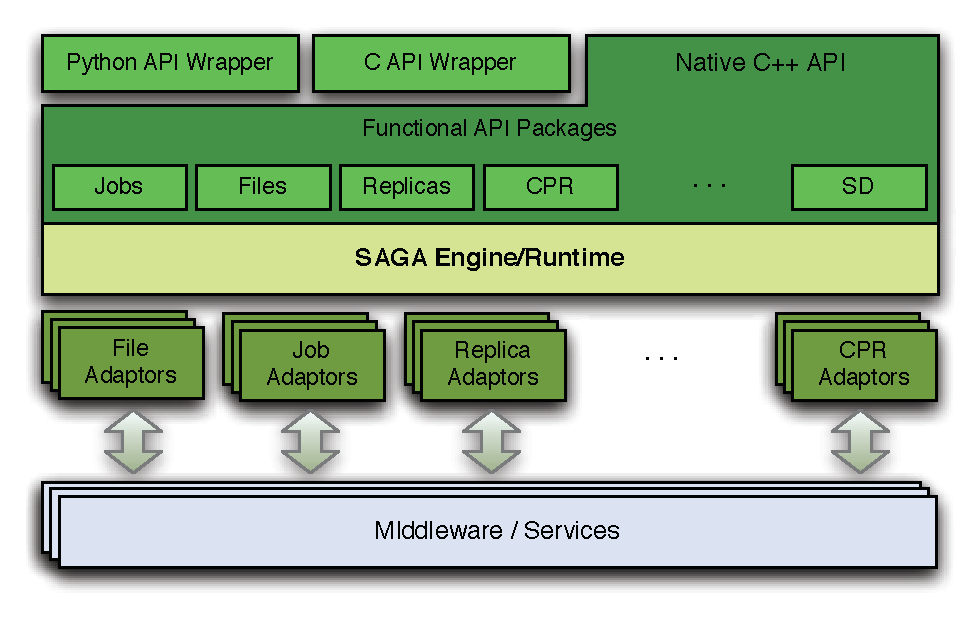
\includegraphics[width=0.40\textwidth]{stci_saga_figures-1.pdf}
 \end{center}
\caption{\small Layered schematic of the different components of the
   SAGA landscape. At the topmost level is the simple integrated API
   which provides the basic functionality for distributed
   computing. Our BigJob abstraction is built upon this SAGA layer
   using Python API bindings.\up} \label{Fig:SAGA1}
\end{figure}

\begin{itemize}
\item File package - provides methods for accessing local and remote
 filesystems, browsing directories, moving, copying, and deleting
 files, setting access permissions, as well as zero-copy reading and
 writing.
\item Job package - provides methods for describing, submitting,
 monitoring, and controlling local and remote jobs. Many parts of
 this package were derived from the largely adopted
 DRMAA specification. 
% ~\cite{drmaa_url} 
\item Other Packages, such as the RPC (remote procedure call), Replica
  package and Stream Package.  remote socket connections with hooks to
  support authorization and encryption schemes.
\end{itemize}

In the absence of a formal theoretical taxonomy of distributed
applications, Fig.~\ref{Fig:sagaapps} can act a guide.  Using this
classification system, there are three types of distributed
applications: (i) Applications where local functionality is swapped
for distributed functionality, or where distributed execution modes
are provided.  A simple but illustrative example is %an ensemble of
an application that uses distributed resources for bulk
submission. Here, the application remains unchanged and even unaware
of its distributed execution, and the staging, coordination, and
management are done by external tools or agents. Most applications in
this category are classified as implicitly distributed.  (ii)
Applications that are naturally decomposable or have multiple
components are then aggregated or coordinated by some unifying or
explicit mechanism.  DAG-based workflows are probably the most common
example of applications in this category.  Finally, (iii) applications
that are developed using frameworks, where a framework is a generic
name for a development tool that supports specific application
characteristics (e.g., hierarchical job submission), and recurring
patterns (e.g., MapReduce, data parallelism) and system functionality.
SAGA has been used to develop system-level tools and applications of
each of these types.

\begin{figure}[!ht]
  \begin{center}
    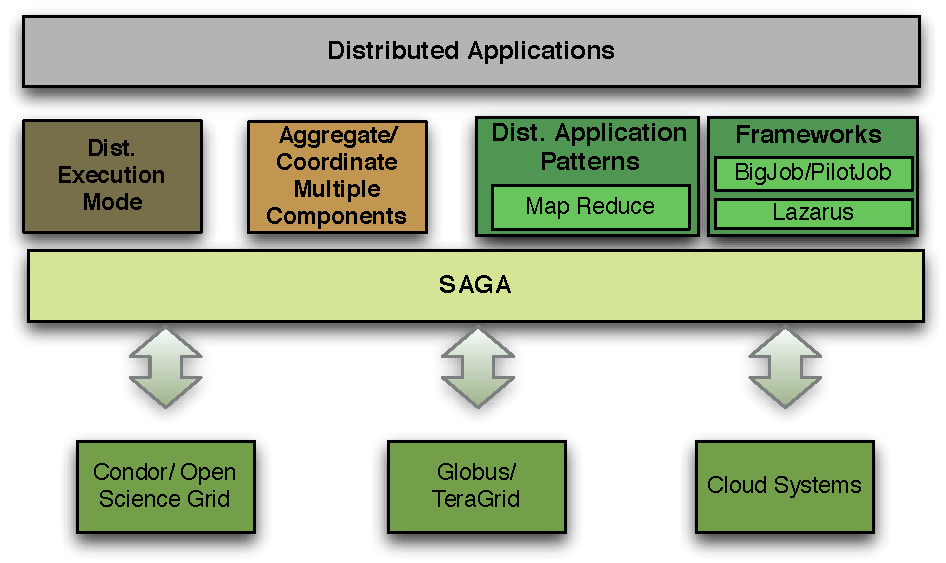
\includegraphics[width=0.45\textwidth]{distributed_applications_saga_figure.pdf}
  \end{center}
  \caption{\small Showing the ways in which SAGA can be used to
    develop distributed applications.  The different shaded box
    represent the three different types; frameworks in turn can
    capture either common patterns or common application
    requirements/characteristics. \label{Fig:sagaapps} \up}
\end{figure}

It is important to note that SAGA provides the basic API to implement
distributed functionality required by applications (typically used
directly by the first category of applications), and is also used to
implement higher-level APIs, abstractions, and frameworks that, in
turn, support the development, deployment and execution of distributed
applications~\cite{enkf-gmac09}. In Ref.~\cite{sagamontage09} we
discussed how SAGA was used to implement a higher-level API to support
workflows. In this paper, we will discuss how SAGA can be used to
implement runtime frameworks to support the efficient execution of the
distributed applications.


\section{Experiments and Analysis}
\up


\subsection{Resources used in Experiments}
\up 

Simulations were performed on a range of supercomputing resources on
TeraGrid machines, shared TeraGrid-LONI (Louisiana Optical Network
Initiative)~\cite{LONI_web} resources and smaller LONI clusters such
as Eric, Oliver, Louie and Poseidon (512 cores).  We also used
Amazon's EC2 and Nimbus as part of the ScienceCloud at Argonne.

\subsubsection*{Resource I: TeraGrid/LONI Cluster (QB)}

To evaluate the performance of BigJob, several experiments have been
conducted on different LONI resources. The resources used are:
QueenBee (QB), Poseidon and Oliver. For accessing these resources
Globus GRAM and an underlying Torque resource manager and Moab
scheduler are used.

\subsubsection*{Resource II: Condor-Pool of LONI Clusters}



\subsubsection*{Resource III: Cloud Environments}

\jhanote{not sure this subsection makes sense. Needs fixing. As does
  the following}

For our experiments we used different Cloud environments: the Nimbus
Science Cloud of the University of Chicago and the Amazon EC2
environment is used. In general, each Cloud has its
characteristics. The Nimbus Cloud is accessed via the WSRF interface,
while for EC2 the Amazon command line client is used. Each Nimbus VM
provides 2 virtual cores and 3.7\,GB memory.  Amazon offeres different
VM types with up to 8 cores. We used the largest VM type (m2.4xlarge)
with 8 cores and 68.4\,GB of memory and the m1.large instance type
with 2 cores and 7.5\,GB, which compares best to the virtual machine
provided by Nimbus.

\subsection{Performance Overheads} 
\up



Interestingly for the experiments conducted, the startup times for the
Cloud environments were observed to be larger than queue-waiting time
for the LONI resource Poseidon, which coincidentally was very lightly
loaded during the course of these experiments. Obviously, the startup
of a VM involves higher overheads than spawning a job on an already
running machine: a resource for the VM must be allocated, the VM must
be staged to the target and booted up. The following experiments will
also show that especially the already oversubscribed intra Cloud
network and thus, the staging of the VM can be a bottleneck. Also,
there is a large fluctuation in particular in the EC2 environment
probably caused by the fact that insufficient resources were available
at certain times.


\section{Conclusion and Future Directions}


\begin{acknowledgement} 
  \up \footnotesize{Important funding for SAGA has been provided by
    the UK EPSRC grant number GR/D0766171/1 (via OMII-UK) and HPCOPS
    NSF-OCI 0710874. SJ acknowledges the e-Science Institute,
    Edinburgh for supporting the research theme, ``Distributed
    Programming Abstractions'' and theme members for shaping many
    important ideas. This work has also been made possible thanks to
    the internal resources of the Center for Computation \& Technology
    at Louisiana State University and computer resources provided by
    LONI. We thank Yaakoub El Khamra for help with initial experiments
    with the Condor infrastructure. We thank Joohyun Kim (CCT) for
    assistance with the RNA models. We thank FutureGrid and
    ScienceCloud for Nimbus resources.}
\end{acknowledgement}

\up
\bibliographystyle{IEEEtran}
\bibliography{literatur,saga}
\end{document}





% \up \up

% \section*{Structure/Outline}

% Section 1. Introduction -- talk about (i) Distributed Systems, need
% for abstractions (development, deployment and execution) and
% programming systems. (ii) Talk about Pilot-Jobs as one of the most
% successful ``execution abstraction''. (iii) Talk about limitations
% of current approaches. (iv) In a nutshell what this paper aims to
% achieve and then conclude with an outline.

% \bigskip

% Section 2. SAGA-based Pilot Job.  SAGA in brief. Place canonical SAGA
% picture. Talk about why using SAGA for PilotJob is different
% (integrated and consistent API). Talk about SAGA Job-Model; talk about
% extensions to the SAGA Job Model for BigJob.  Architecture and Control
% Flow for BigJob. Discuss how SAGA BigJob works well with Condor
% Glide-in.

% \bigskip 

% Section 3. Introduce Clouds -- SAGA for Clouds and parallel jobs for
% Clouds. Explain the role of a Pilot Job for Clouds. What does it mean?
% How is it different from Pilot Jobs for Grids/Clusters?  Talk about
% Parallel jobs and Clouds and how we manage them.

% \bigskip 

% Section 4. Usage Modes and Analysis: Already laid out.

% \bigskip 

% Section 5. Conclusion

% \jhanote{We need to be consistent with the usage of sub-job and
%   Sub-Job and subjob/SubJob. Preference?}

% \alnote{What spelling convention should we use: Pilot-Job, Big-Job,
% Sub-Job or PilotJob, BigJob, SubJob?}

% There is a perception that developers also prefer to ``roll out their
% own" capabilities, even though there exist programming systems with
% similar capabilities..

% Viewed alternatively, the capability of infrastructure -- as defined
% by the tools, programming systems and policy determine applications,
% type development \& execution

% This may be due to a number of factors: Many programming systems lack
% robustness when used by developers in scientific applications -- for
% instance, they may have limits on scalability. It may be difficult to
% isolate a specific capability from a programming system, thereby
% limiting re-use by an application developer requiring that
% capability. In general~\cite{dpagrid2009} programming systems fall
% short of the requirements of distributed applications due to: {\em
%   i. Incompleteness:} Programming systems and tools are often
% incomplete or inflexible with respect to application needs, e.g.,
% tools that support the master-worker paradigm often only address
% failures of workers and not of the master. {\em ii. Customization:}
% Programming systems and tools also tend to be customized to
% applications and their requirements, with limited concern for reuse or
% extensibility.  Applications and tools are also often highly dependent
% on (and tuned to) a specific execution environment, further impacting
% portability, re-usability, and extensibility.
